\documentclass{article}[11pt]
\textheight 8.5in
\usepackage{graphicx}
\usepackage{float}%for forcing position of figs
\usepackage{hyperref}


\begin{document}
\begin{center}
Siddharthan Rajasekaran\\
Week of 2/27/2017 - 3/6/2017
\end{center}

\section{Summary of Discussions}
We will talk about why and when to use Deep learning with RL also called Deep Reinforcement Learning (DRL). Also introduce transfer learning in DRL setting.

\section{Deep Learning}
Lately, in many domains including vision, control, model fitting ... etc we have started to use Deep neural networks. They are just a good and practically reliable tool to do function approximation. Deep neural nets are just a composition of many functions. Each function is defined as a layer in the architecture. The output of a layer is just some function (linear or non-linear) of linear combinations of outputs from the previous layer. The same follows recursively to get the required output. Given an input sample, after learning, we feed the input to the first layer whose output will be the inputs of the next layer. Hence the out put is a compounded function of the input. It is common to define the loss function as the squared error between the prediction and the labels. Since the neural network is just a parametrized function of $w$ (free parameter) we are allowed degrees of freedom in the space of $w$ to reach minimum error. So to compute the gradient to perform a gradient descent, one just follows the chain rule and unrolls the recursive gradient estimation backwards from the last layer. This is shown in figure.\ref{fig:backprop}. The gradient at the last layer is given in figure.\ref{fig:lastlayer}

\begin{figure}[H]
  \begin{center}
    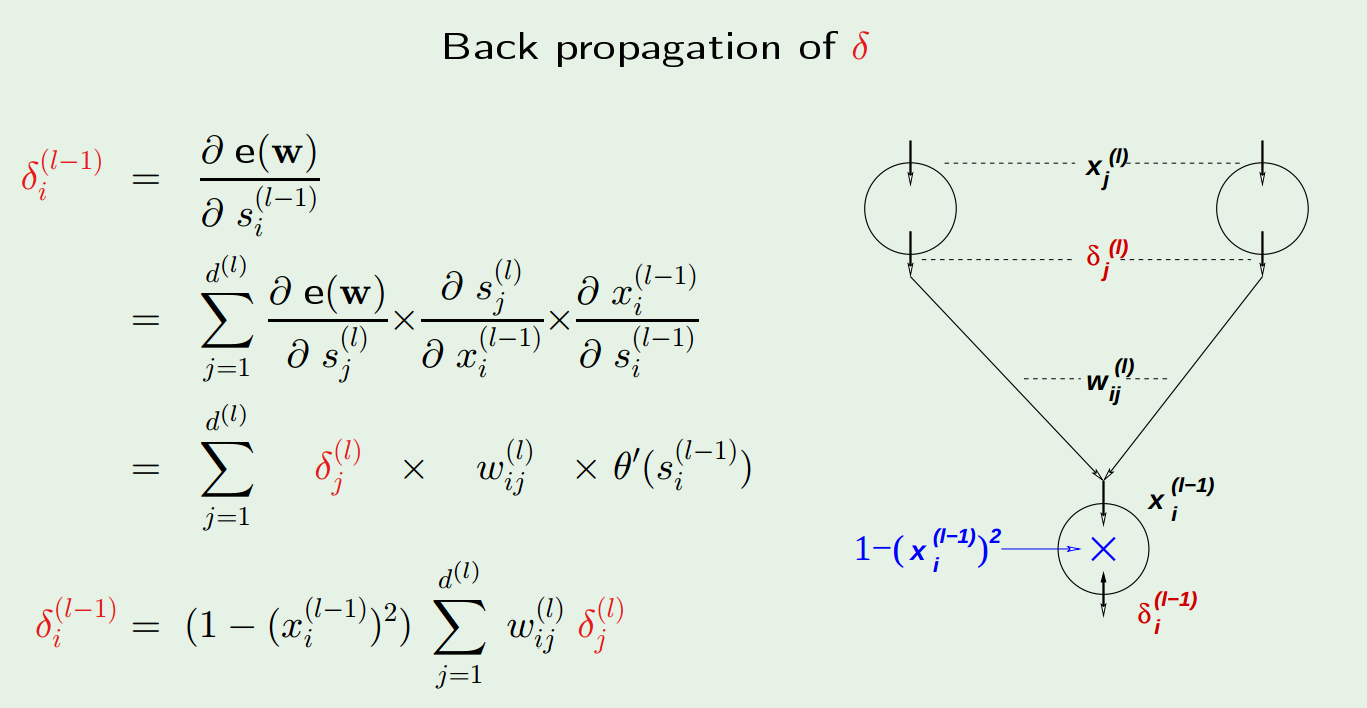
\includegraphics[width=1\linewidth]{images/backprop}
    \caption{Back propagating gradients in a neural network}
    \label{fig:backprop}
  \end{center}
\end{figure}

\begin{figure}[H]
  \begin{center}
    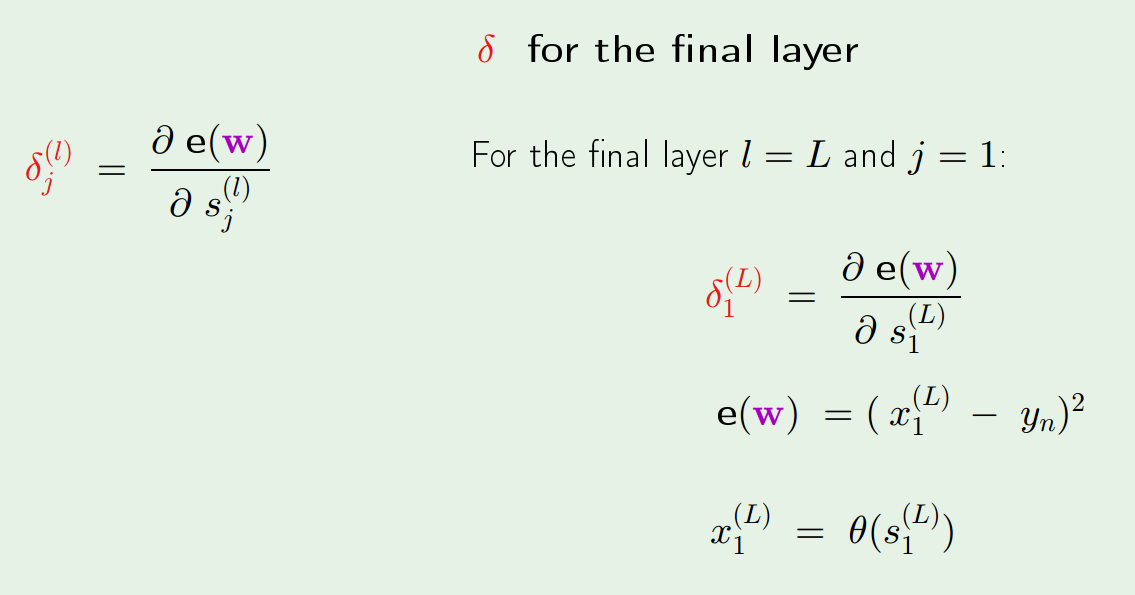
\includegraphics[width=1\linewidth]{images/lastlayer}
    \caption{Gradient of the error in th elast layer}
    \label{fig:lastlayer}
  \end{center}
\end{figure}

\section{RL}
RL can be solved using three methods 1) Value based, 2) Policy based, 3) Model Based. We saw how in MDP settings, solving the RL problem using Q values (1) requires solving the Bellman's equation (Bellman update in DP shown in figure \ref{fig:bellman}). 

In 2) We just parametrize the policy itself then we try and search directly those parameters using evolution based algorithms or policy gradients (Week 1 report) 

In 3) We build a model of the environment and solve RL using Value iteration ... etc

\begin{figure}[H]
  \begin{center}
    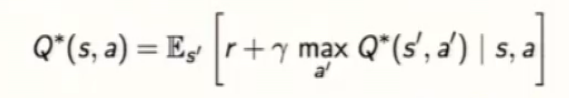
\includegraphics[width=0.5\linewidth]{images/bellman}
    \caption{Bellman equation}
    \label{fig:bellman}
  \end{center}
\end{figure}

Let us discus use of DNN in solving RL using 1). It is often hard to compute Q values until convergence (in case of recursive DP). Especially because we have to max over the possible actions. This becomes exponentially more expensive with the number of states. One way to solve this would be to perform Q-approximation. One can imagine Q value of a state to be weighted features. This will be a linear Q function. However to represent complex The value functions are represented by what are called as Q networks. The input to these networks is state $s$ and $a$ and the output is $Q$ values. The error function is given by the bellman update equation as shown in figure \ref{fig:error}. 

\begin{figure}[H]
  \begin{center}
    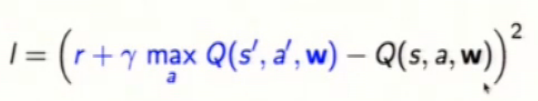
\includegraphics[width=0.5\linewidth]{images/error}
    \caption{Error function in Q-networks}
    \label{fig:error}
  \end{center}
\end{figure}

This makes it extend well to high dimensional spaces and approximates non-linear reward functions. Which is out case in manipulation tasks. 

\section{Transfer Learning}
Most literature in LfD requires different demonstrations for completing different tasks. For example consider pick and place task in which a robot has to move an object from region 1 or 2. For different objects, we need different demonstrations because the way we might manipulate it could be different. Hence the process of learning from new demonstrations is slow. One can generalize and transfer knowledge from one domain to another. 

Transfer Learning literature has some metrics to evaluate the amount of transfer \cite{taylor2009transfer}.

\begin{itemize}
\item Jumpstart: The initial performance of an agent in a target task may be improved by transfer
from a source task.
\item Asymptotic Performance: The final learned performance of an agent in the target task may be
improved via transfer.
\item Total Reward: The total reward accumulated by an agent (i.e., the area under the learning
curve) may be improved if it uses transfer, compared to learning without transfer.
\item Transfer Ratio: The ratio of the total reward accumulated by the transfer learner and the total
reward accumulated by the non-transfer learner.
\item Time to Threshold: The learning time needed by the agent to achieve a pre-specified performance
level may be reduced via knowledge transfer
\end{itemize}

Transfer learning is not an alien concept in machine learning/ reinforcement learning. For instance there has been several works to transfer the Q values of one MDP to another based on the similarity of states \cite{glatt2016towards}. Defining a hand engineered similarity metric is often common. However, since there is also literature on warping functions which essentially transforms demonstrations to a space where they are comparable to make state-wise association (using time maybe), can we use these warping functions to find similarity metric and hence transfer Q values. More interestingly, can we use neural nets to approximate these warping functions by formally learning in several source and target tasks?   
More importantly, will the jumpstart policy allow us to learn policy in the new domain without new demonstration? This jumpstart policy should let the agent explore near promising regions which will result in completion of the new task given new reward functions. 


 




\section{Bibliography}

\bibliographystyle{plain}
\bibliography{bibfile}
\end{document}
